\documentclass[14pt]{article}

\usepackage[letterpaper,margin=0.75in]{geometry}

\usepackage[outputdir=../dist]{minted}

\usepackage{amsmath}
\usepackage{booktabs}
\usepackage{graphicx}
\usepackage{listings}
\usepackage{fancyhdr}
\usepackage{standalone}
\usepackage{float}
\usepackage{hyperref}
\usepackage[style=vancouver]{biblatex} %Imports biblatex package

% Bibliography
\addbibresource{all.bib}

% \include{data/reaction-time.csv}
 
% \pgfplotsset{compat = newest}

\setlength{\parindent}{0pt}

\pagestyle{fancy}

\begin{document}

\lstset{
  language=Python,
  basicstyle=\small,          % print whole listing small
  keywordstyle=\bfseries,
  identifierstyle=,           % nothing happens
  commentstyle=,              % white comments
  stringstyle=\ttfamily,      % typewriter type for strings
  showstringspaces=false,     % no special string spaces
  numbers=left,
  numberstyle=\tiny,
  numbersep=5pt,
  frame=tb,
}

\title{PX2505 - Electronics Lab Report - Haunted Doll Factory }
\date{}
\def\theinstructor{}



\author{Sidney Pauly}
\def\theuoastudentid{52104132}

\makeatletter

\let\thetitle\@title
\let\theauthor\@author
\let\thedate\@date


\makeatother




\fancyhf{}
\fancyhead[L]{\today}
\fancyhead[C]{Name: \theauthor}
\fancyhead[R]{ID: \theuoastudentid}

\fancyfoot[C]{\thepage}
% \maketitle

\begin{titlepage}
  \begin{center}
    \Large
    \textbf{\thetitle}
        
    \vspace{0.4cm}
    \large
    \thetitle
        
    \vspace{0.4cm}
    \textbf{\theauthor}\\
    \textbf{\theuoastudentid}\\
    \textbf{\today}\\

       
    \vspace{0.9cm}
    \textbf{Declaration}\\
    I certify that this report has been written by myself, except where otherwise
    indicated
  \end{center}

  \vfill

  \begin{center}

    University of Aberdeen\\
    Scotland\\
    UK\\
    \thedate
    \vspace{0.4cm}
    \url{https://github.com/sidney-pauly/papers}
  \end{center}
\end{titlepage}

\tableofcontents

\section{Introduction}

The electronics section of the PX2505 course focuses on digital logic or TTL (Transistor-transistor logic). Broadly speaking the aim of digital logic is to perform logic
operations to perform various practical tasks. The most simple case is to directly evaluate logical conditions electronically. An example could
be a traffic light assembly: The light for the pedestrians should only be set to green if the request button is pressed and no car is currently
on the intersection, but not if it was already green in the last 30s. Those conditions can be translated into formal logic and further into
a digital circuit which then performs these operations. In principle digital logic circuits can execute any higher order algorithms, which is what computers do,
However this experiment only focuses on simple logic like in the example. The aim will be to analyze the requirements set out, build a schematic
version of the circuit and finally a physical working version of the same.\\
\\
The "Haunted Doll Factory" is exactly about such an application of basic logic. The doll has four inputs and four outputs and the task is to 
have the motors (outputs) only turn on when specific inputs are active. Using simple logic gates (AND, OR, XOR, etc.) these requirements can be implemented
both as an actual circuit as well as a simulation one (with the Multisim simulation tool)\\
\\
A further practical goal when building digital circuits is to achieve the requirements with as little components as possible. This is because fever components
reduce the amount of failure points as well as the energy consumption of the device. To reduce the amount of components while still achieving the
same logical behavior analytical methods can be used. Boolean algebra is a mathematical description of logic and can therefore be used
to manipulate logical statements and to reduce them to their simplest form. This technique was used in this experiment to greatly reduce the 
number of required logic gates.

\section{Experiment}

\subsection{Aim}

The Lab Manual\autocite{ross} sets out the following scenario: We are tasked with designing an electronic circuit, that controls the behavior of a (haunted) doll.
The doll has four inputs (those could be buttons or switches) and four outputs (motors that can either be turned on or off). The desired logical
behavior of how these inputs and outputs are related is given by (Table \ref{table:desired-behaviour}):


\begin{table}[H]
  \centering
  \begin{tabular}{llll|llll}
  \multicolumn{4}{l}{INPUT} & \multicolumn{4}{l}{OUTPUT} \\
  $S_1$ & $S_2$ & $S_3$ & $S_4$ & $M_1$ & $M_2$ & $M_3$ & $M_4$ \\
  \hline
  0    & 0    & 0    & 0    & 0     & 0    & 0    & 0    \\
  0    & 0    & 0    & 1    & 0     & 0    & 0    & 1    \\
  0    & 0    & 1    & 0    & 0     & 0    & 1    & 0    \\
  0    & 0    & 1    & 1    & 0     & 0    & 0    & 0    \\
  0    & 1    & 0    & 0    & 0     & 0    & 0    & 0    \\
  0    & 1    & 0    & 1    & 0     & 0    & 0    & 0    \\
  0    & 1    & 1    & 0    & 0     & 0    & 0    & 0    \\
  0    & 1    & 1    & 1    & 0     & 0    & 0    & 0    \\
  1    & 0    & 0    & 0    & 1     & 0    & 0    & 0    \\
  1    & 0    & 0    & 1    & 1     & 0    & 0    & 1    \\
  1    & 0    & 1    & 0    & 1     & 0    & 1    & 0    \\
  1    & 0    & 1    & 1    & 0     & 0    & 0    & 0    \\
  1    & 1    & 0    & 0    & 1     & 1    & 0    & 0    \\
  1    & 1    & 0    & 1    & 0     & 0    & 0    & 0    \\
  1    & 1    & 1    & 0    & 1     & 1    & 1    & 0    \\
  1    & 1    & 1    & 1    & 0     & 0    & 0    & 0   
  \end{tabular}
  \caption{\label{table:desired-behaviour} Desired Behavior of the Doll \autocite{ross}}
\end{table}

$S_{1-4}$ specify the four inputs, while $M_{1-4}$ specify the four outputs (motors). If a given input shows 0 its off, if it shows 1 its on, the same applies
to the motors.

\subsection{Theory}
At first glance the behavior of the doll looks quite complex. It is not immediately clear what sort of simple logical expression could describe
the behavior of the doll in its entirety. Luckily there are tools to analyze such requirements and thus arrive at a simplified expression.\\

The first thing that could be asked is for what inputs a motor is on? This can then be translated into logical language
and those logical expression can then be reduced. A simple example is Motor 2, it is on if input 1 is on, input 2 is on, input 3 is off and input 4 is off.
Alternatively it is also on if input 1 is on, input 2 is on, input 3 is on and input 4 is off. For all other cases the motor is off. This can also
be represented in boolean algebra:
$$
M_2 = (S_1*S_2*\bar{S_3}*\bar{S_4}) + (S_1*S_2*S_3*\bar{S_4})
$$
Translated to natural language multiplication means "and", addition "or" and a bar over the respective value means "not". The nice thing about this
representation is that relevant algebraic rules hold, i.e. transitivity, commutativity, etc.\autocite{ross}.\\

Thus the above expression can be simplified to:
$$
M_2 = (S_1*S_2*\bar{S_4})(S_3+\bar{S_3})
$$

as something OR not something ($ X + \bar{X} $) is always true the expression further simplifies to:

$$
M_2 = S_1*S_2*\bar{S_4}
$$

Through the same technique similar expressions for the other motors could be derived. Then the expressions could be compared and
similar operations could then be implemented with the same physical components to reduce their overall count.\\

However in case of the doll there is a quicker and more effective way: converting the binary input and output signals to decimal. 
As we are more used to decimal (and because decimal represents more information in fever digits) it is sometimes more intuitive to understand 
and to infer patterns. Table \ref{table:decimal} shows such a decimal translation. The representation
treats every input as a digit of a four digit binary number. The same is done for the output.

\begin{table}[H]
  \centering
  \begin{tabular}{lll}
  Input                       & Active Motor        & Output \\ 
  \hline
  0                           &                     & 0      \\
  1                           & $M_4$               & 1      \\
  2                           & $M_3$               & 2      \\
  3                           &                     & 0      \\
  4                           &                     & 0      \\
  5                           &                     & 0      \\
  6                           &                     & 0      \\
  7                           &                     & 0      \\
  8                           & $M_1$               & 8      \\
  9                           & $M_1$, $M_4$        & 9      \\
  10                          & $M_1$, $M_3$        & 10     \\
  11                          &                     & 0      \\
  12                          & $M_1$, $M_2$        & 12     \\
  13                          &                     & 0      \\
  14                          & $M_1$, $M_2$, $M_3$ & 14     \\
  15                          &                     & 0     
  \end{tabular}
  \caption{\label{table:decimal} The behavior translated to Decimal}
\end{table}

Doing this translation immediately makes it obvious that there are just two cases:
\begin{enumerate}
  \item The output is 0 (all motors are off)
  \item The input is the same as the output (the motors belonging to the respective input are on) 
\end{enumerate}

The result of this realization is that the task can be rephrased: we need a circuit that is only on for the binary representations of the
numbers 1, 2, 8, 9, 10, 12 and 14. The most direct (but also most inflated) boolean representation of the same is this:

$$
F = (\bar{S_1}\bar{S_2}\bar{S_3}S_4)+(\bar{S_1}\bar{S_2}S_3\bar{S_4})+(\bar{S_1}\bar{S_2}S_3\bar{S_4})+(S_1\bar{S_2}S_3S_4)+(S_1\bar{S_2}S_3\bar{S_4})+(S_1S_2\bar{S_3}\bar{S_4})+(S_1S_2S_3\bar{S_4})
$$

Through a lot of algebraic manipulation one can end up with the following expression:

$$
F = S_1\bar{S_4} + \bar{S_2}S_3\bar{S_4}+\bar{S_2}\bar{S_3}S_4
$$

This expression can be further simplified by using the fact that $X\bar{Y}+\bar{X}Y = X \oplus Y$, i.e. X and not Y or not X and Y is the same
as only X or only Y (exclusive OR):

\begin{equation}
F = S_1\bar{S_4} + \bar{S_2}(S_3 \oplus S_4)
\label{eq:logic_filter}
\end{equation}

This simple expression now distinguishes the two cases laid out previously. If the expression is false, no motors should be on. If it is true
the motors which have their corresponding input on should be on. Algebraically this can be expressed as 
\begin{equation}
M_n = S_nF
\label{eq:apply_filter}
\end{equation}

Note that this expression basically acts as a filter or mask on
the inputs. Because of this the expression will from now on be referred to as the logic filter.


\clearpage
\subsection{Verifying the theory}

Before spending a lot of time on building circuits it useful to know that the discoverd logic expression does indeed recover the desired logical behavior.
The following script runs through all different input combinations and applies the logical expression to them. The result is then printed out.

\begin{minted}[linenos]{python}
import pandas as pd

result = [0] * 16

for i in range(0, 16):

    # Decimal to binary digit conversion
    s_1 = (8 & i) > 0
    s_2 = (4 & i) > 0
    s_3 = (2 & i) > 0
    s_4 = (1 & i) > 0
    
    # Calculate the logic filter
    F = (s_1 and not s_4) or (not s_2 and (s_3 ^ s_4))

    # Apply the filters to the input and thus produce the output
    result[i] = [s_1, s_2, s_3, s_4, F and s_1, F and s_2, F and s_3, F and s_4]

# Print the result through a pandas data frame to have it formatted
print(pd.DataFrame(result))
\end{minted}

The output of this script matches table \ref{table:desired-behaviour} exactly, confirming that the simplification process worked

\subsection{Schematic Diagram}

The first step is to draw a schematic diagram of the resulting circuit. The following schematic diagram was drawn and then simulated with multisim:

\begin{figure}[H]
  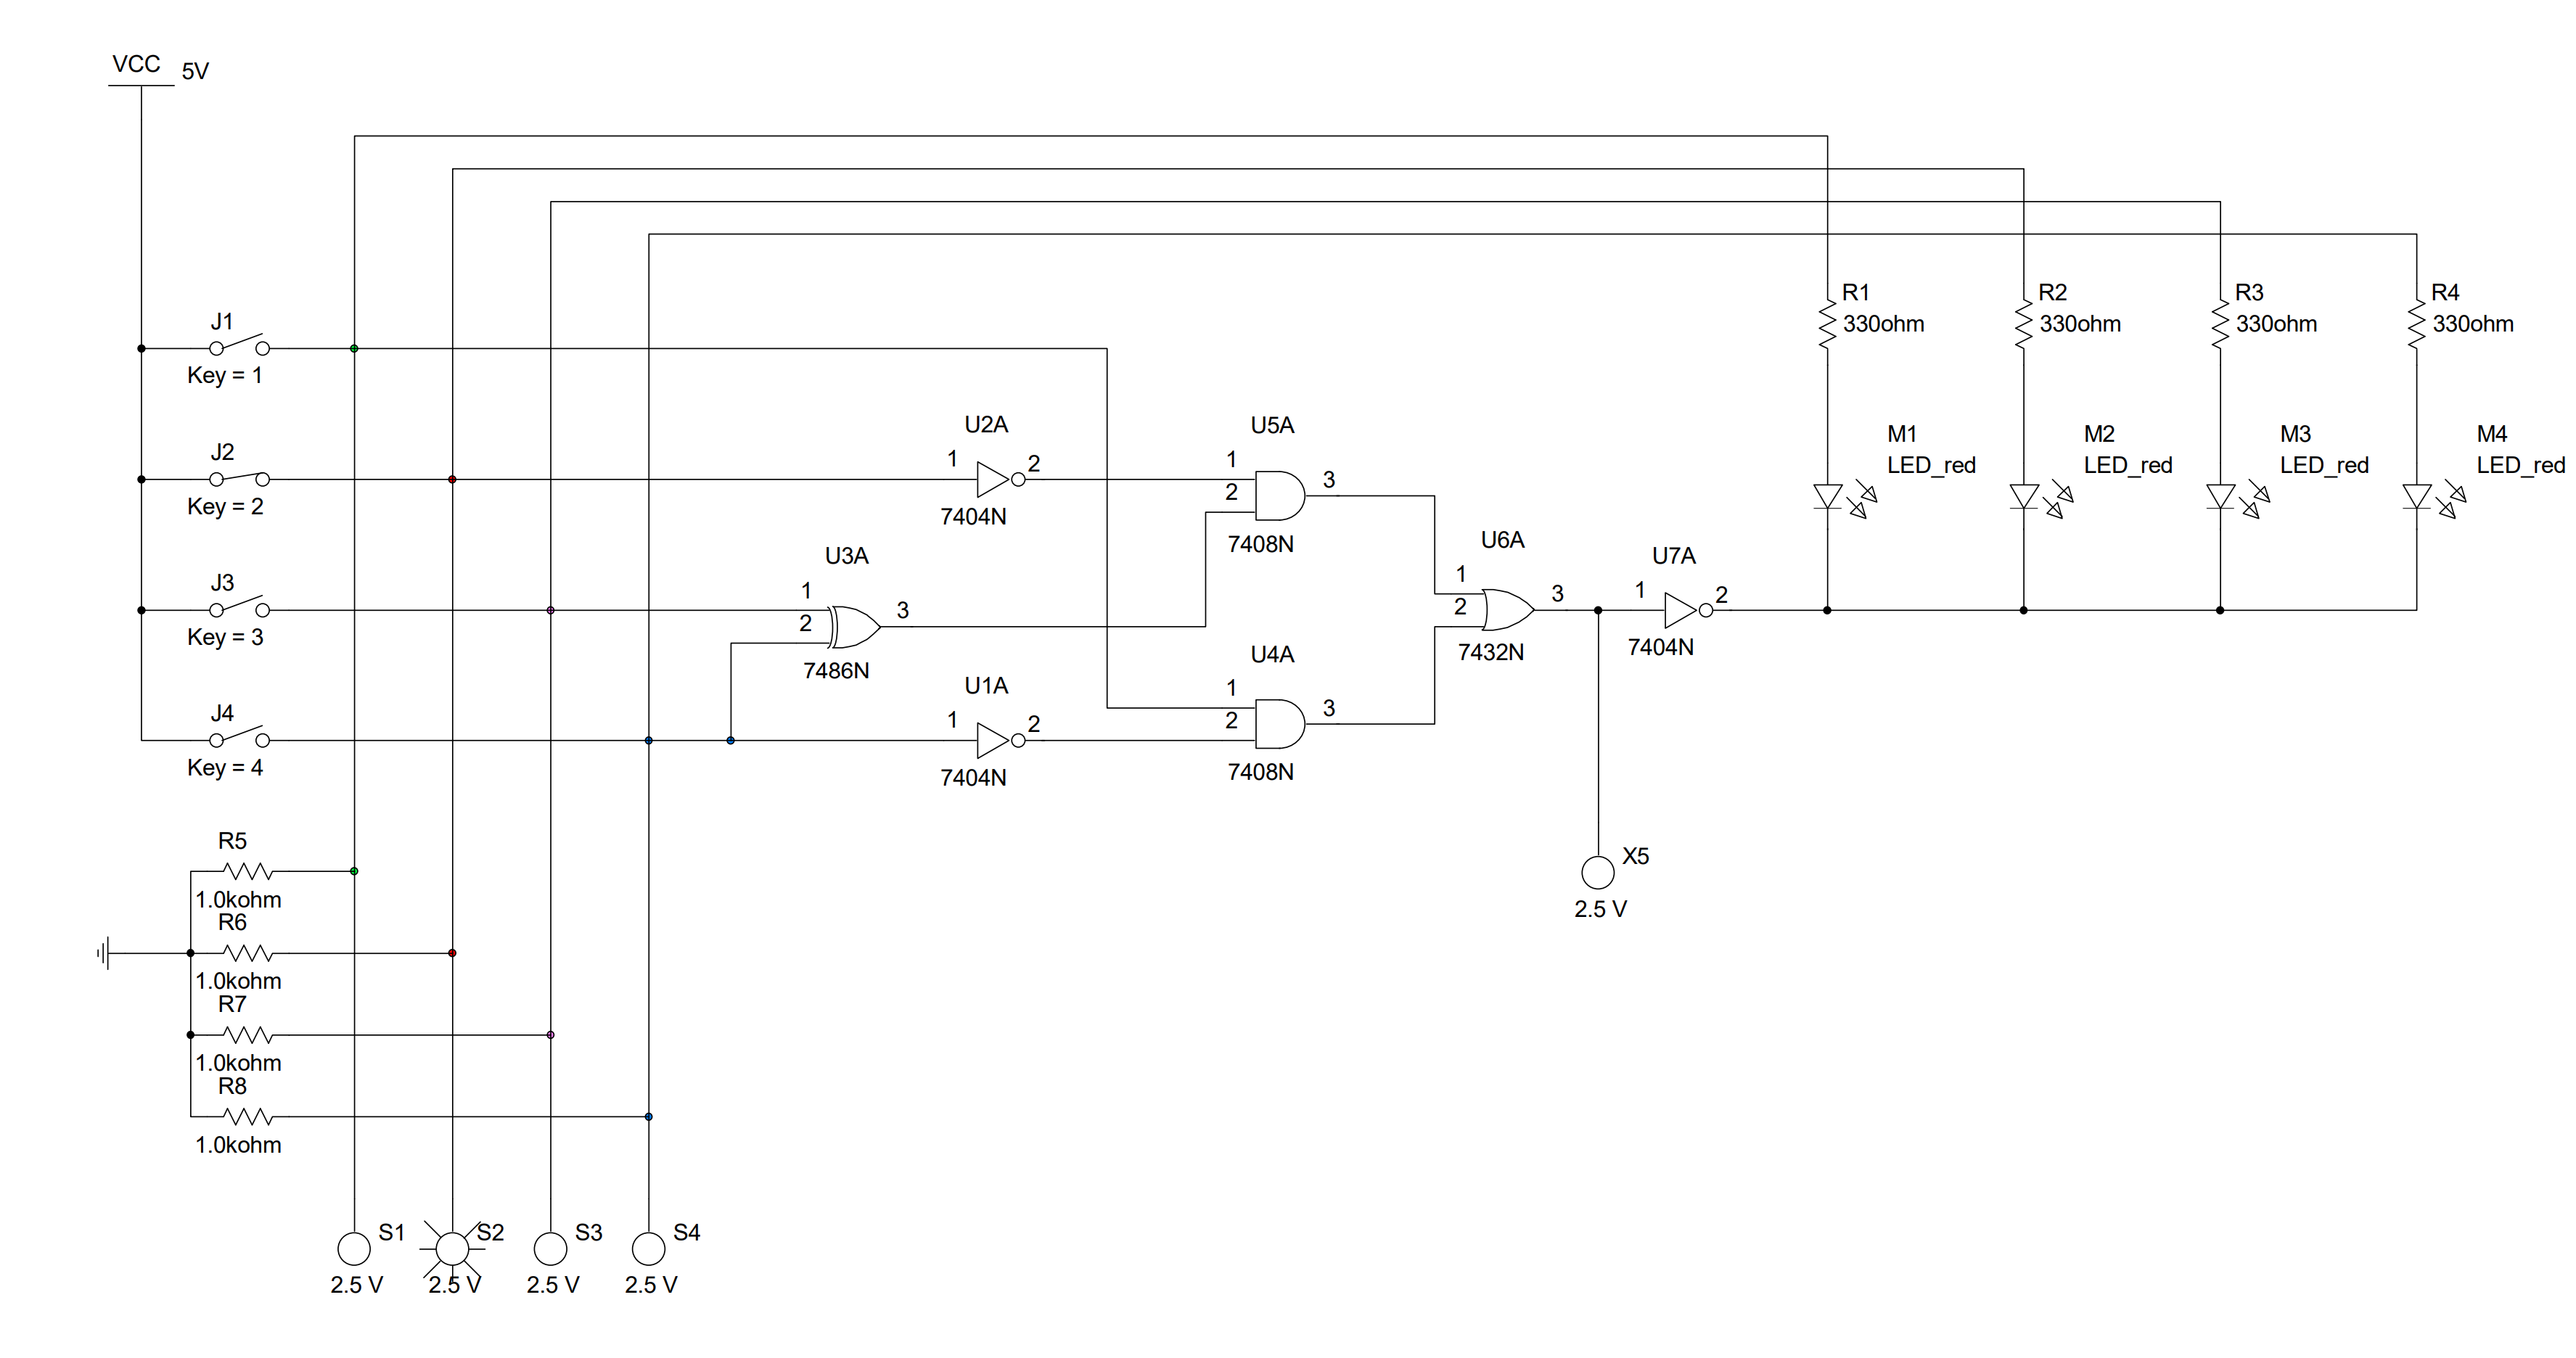
\includegraphics[width=17cm]{./images/schematic.png}
  \caption{Schematic diagram of the "Haunted Doll" circuit}
  \label{fig:schematic}
\end{figure}

The resulting circuit consists of three main sections. Each section has some additional features and optimizations. Because the circuit is designed
with the multi sim software it can be simulated. The circuit showcased in figure \ref{fig:schematic} was tested for all possible inputs of $S_{1-4}$
and yielded the behavior expressed in table \ref{table:desired-behaviour}. 

\subsubsection{Input}
The input section consists of four switches. Each of the switches corresponds to one of the inputs $S_{1-4}$. In the diagram they are labeled with J1-J4.
If the input switches are closed the corresponding wire will be at VCC voltage ($5V$). This voltage (also referred to as HIGH) corresponds to an input value
of 1. A value of 0 is represented by $0V$ (also called GND). Note that the input wires are always connected to GND through a $1k\Omega$ resistor. This connection ensures
that when the input switches are open that the input wire is at a valid logic value of GND. If there would be no connection in that case the corresponding
input would have an undefined value, which could lead to undefined behavior. Connecting the input through a $1k\Omega$ resistor ensures that in case the swtich
is closed the input will be at VCC voltage, as the wire without resistance "overpowers" the connection with resistor. \\

In the schematic additional logic probe indicator lights are attached to the input cables (S1-S4). Their purpose is to quickly and easily
determine the state of the given input.

\subsubsection{Logic}

The logic section takes in the four input signals and proccesses them. The implemented logic corresponds exactly to the logic filter
$F$ (equation \ref{eq:logic_filter}). The logic section ends at the logic probe indicator light (label X5). This light is there to quickly
determine the value of $F$ (the logic filter value). The subsequent inverter (label U7A) is not considered
part of that section. It belongs to the output section and its purpose will be explained subsequently.\\

To implement equation \ref{eq:logic_filter} the corresponding 74xx series TTL logic components are used:

\begin{enumerate}
  \item 7404N Inverter (NOT) 
  \item 7486N XOR 
  \item 7408N AND 
  \item 7432N OR  
\end{enumerate}

The layout corresponds to the equation 1:1. This can be seen easiest going backwards from the OR gate (label U6A). It's lower
input corresponds to the left component of equation \ref{eq:logic_filter} and it's upper input to the right component. Consequently the lower
AND gate (label U4A) has $S_1$ and $\bar{S_4}$ as inputs ($S_4$ gets inverted through inverter U1A). Equally the upper AND gate (label U5A) is
connected to to $\bar{S_1}$ (inverter U2A) and the exclusive or gate (label U3A) that combines $S_3$ and $S_4$.

\subsubsection{Output}

The last section is the output section. It has two tasks, display the result through LEDs ($M_{1-4}$ standing in for the motors) as well as applying 
the logic filter $F$ to the inputs $S_{1-4}$ (Equation \ref{eq:apply_filter}). The obvious way to do the later would be to add another four
AND gates combining $F$ and $S_n$. Instead another trick can be employed here. Because the LEDs are diodes they are only on if they are connected
to HIGH on one side (Anode $A$) and to LOW on the other (Cathode $K$). In any other configuration the LEDs won't turn on. This behavior can be abused as the
LED therefore acts as an AND gate with the equation $O = A\bar{K}$. To emulate the behavior of equation \ref{eq:apply_filter} the filter $F$ simply has
to be inverted and connected to the Cathodes ($K$) (this is why the inverter with label U7A is needed) and the inputs $S_n$ to each of the anodes.\\

To prevent the LEDs from overheating $330\Omega$ current limiting resistors are added in series.

\clearpage
\subsection{The Physical Circuit}

The implemented physical circuit is the direct implementation of the schematic, with some minor modifications for practicality.

\begin{figure}[H]
  \centering
  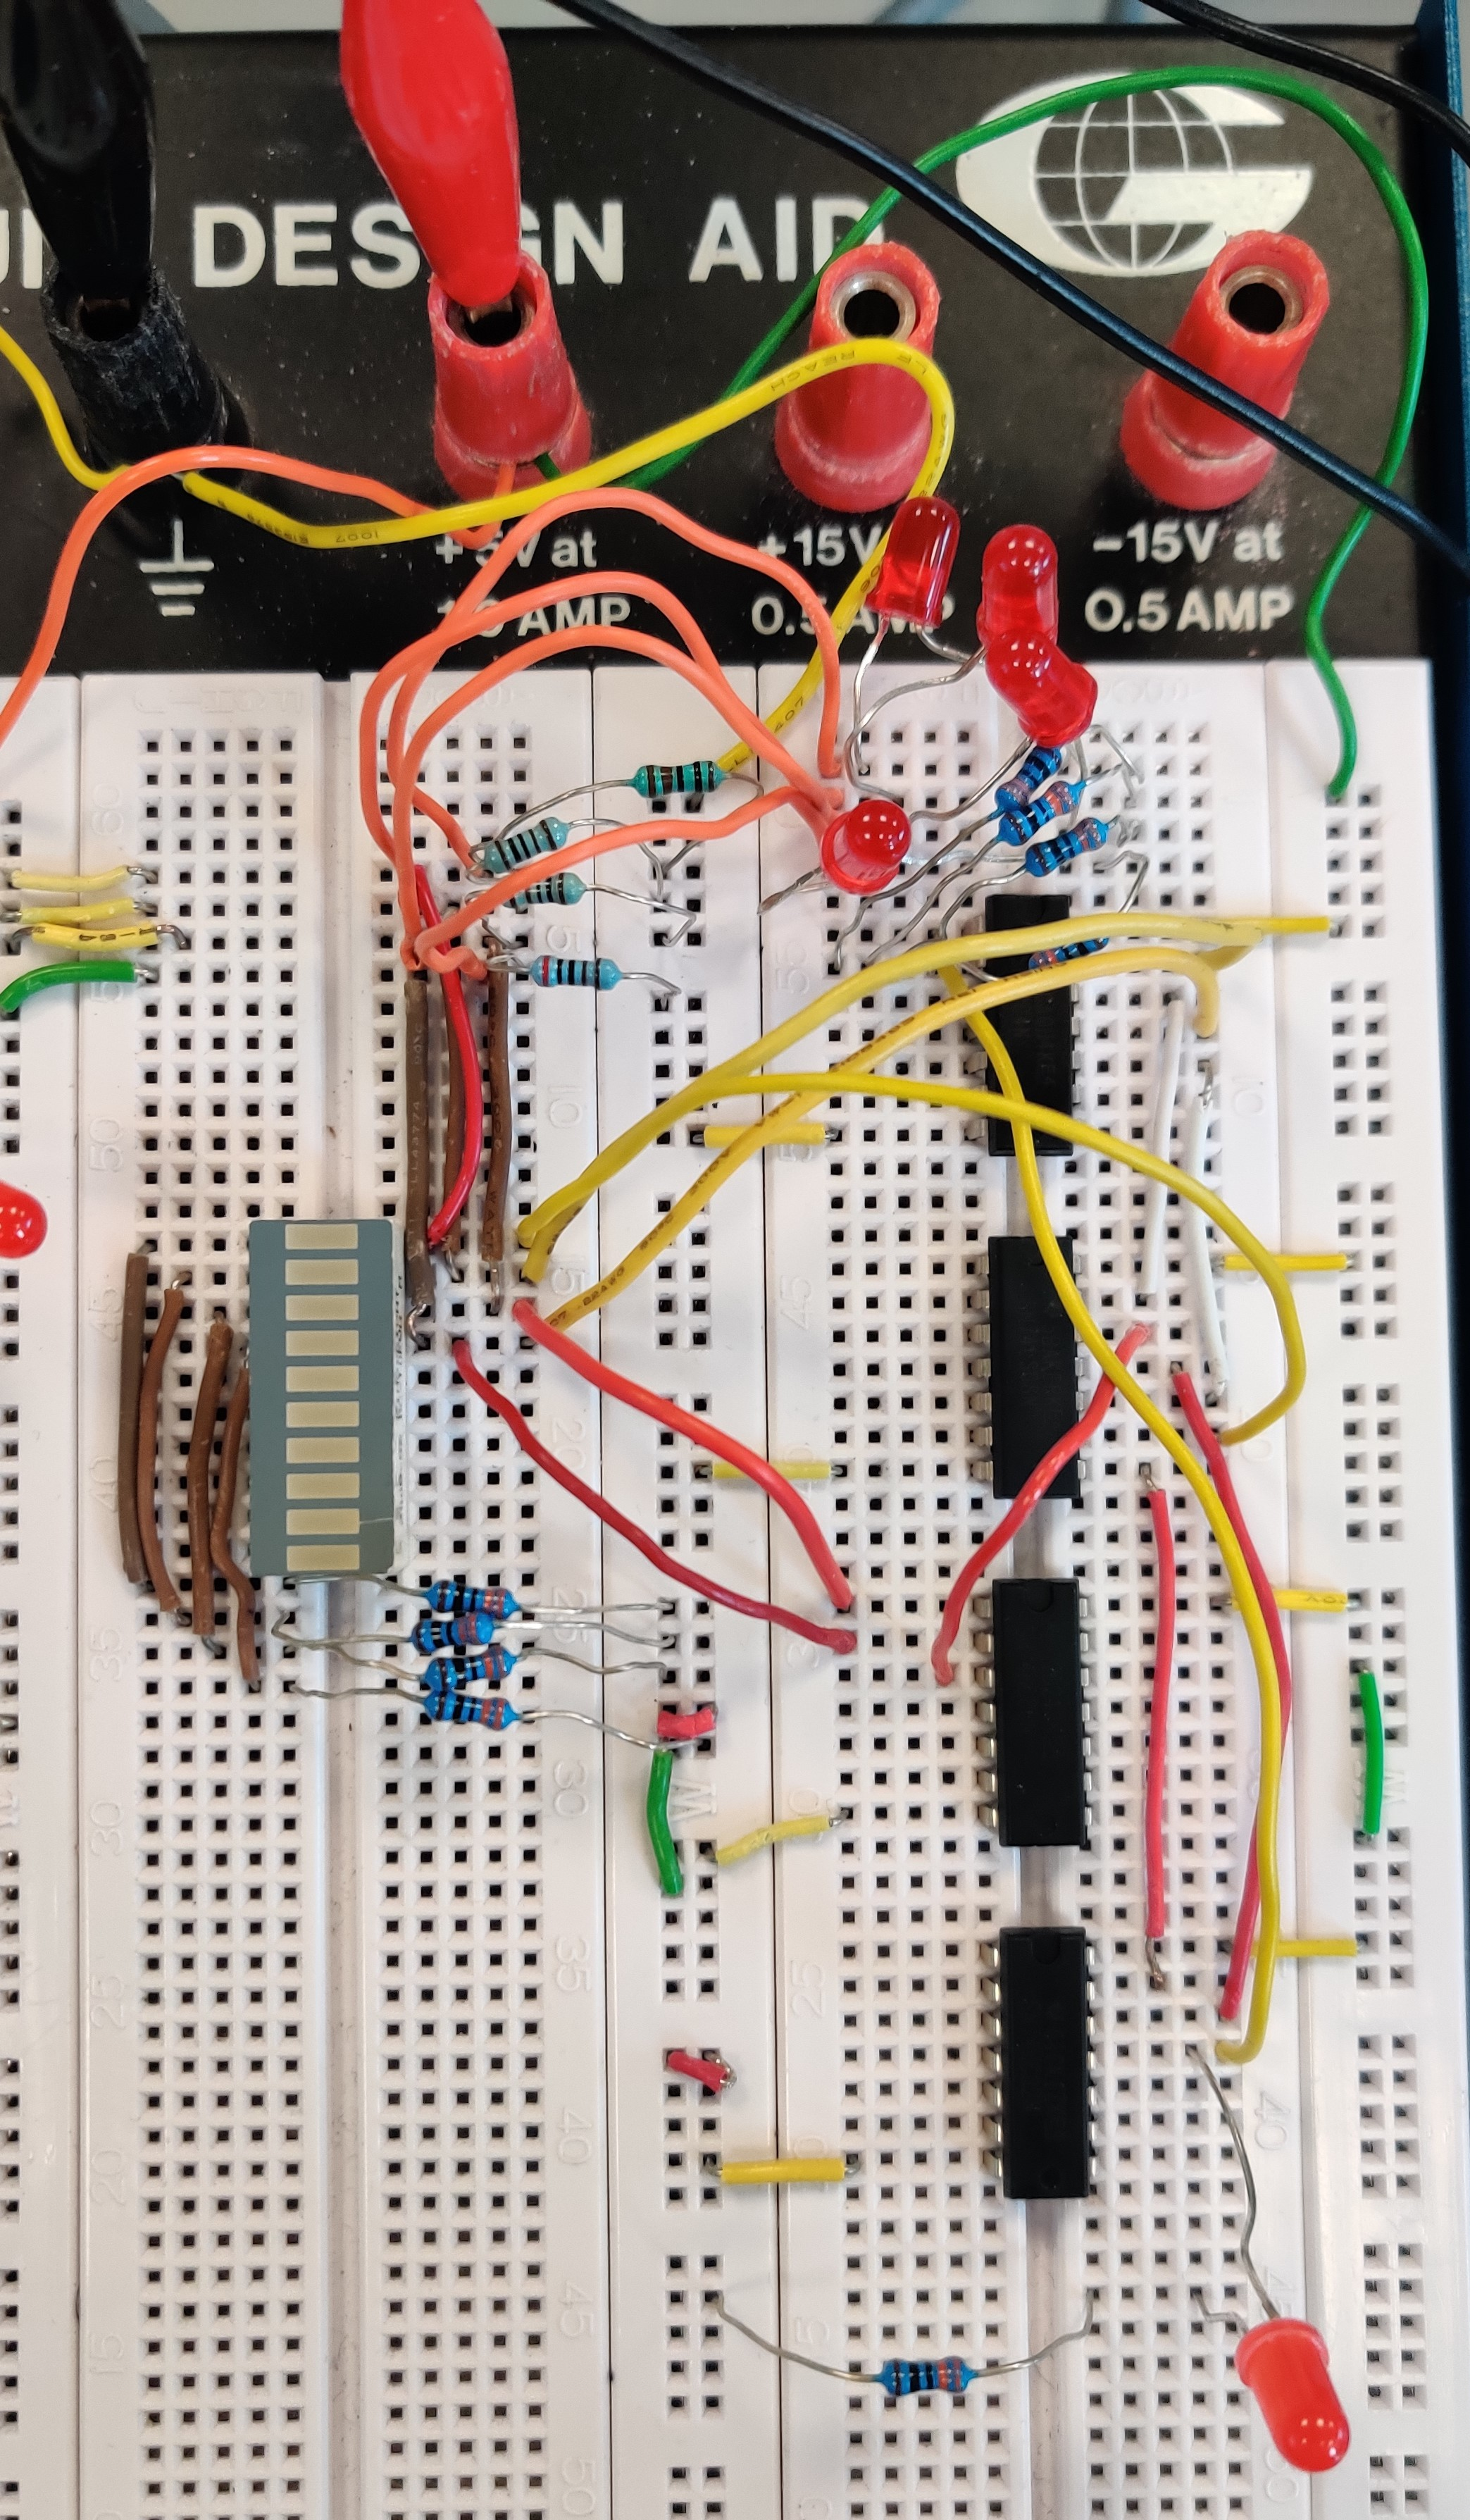
\includegraphics[width=8cm]{./images/circuit.jpg}
  \caption{The physical "Haunted Doll" circuit}
  \label{fig:circuit}
\end{figure}

\subsubsection{Components}

The following components where used in the circuit:

\begin{enumerate}
  \item 1 8-digit LED bar
  \item 5 Red LEDs
  \item 9 $330\Omega$ resistors
  \item 4 $1k\Omega$ resistors
  \item 1 Texas Instruments S7404 Inverter chip\autocite{ti:7404}
  \item 1 Texas Instruments SN74HC86 XOR chip\autocite{ti:7486}
  \item 1 Texas Instruments SN74HC32 OR chip\autocite{ti:7432}
  \item 1 Texas Instruments SN74LS08 AND chip\autocite{ti:7408}
\end{enumerate}

Just like the schematic the physical circuit consists of the same three sections. 



\subsubsection{Input}

The input section covers the left breadboard (Figure \ref{fig:circuit}).
The input section consist of an 8-digit LED bar which shows which of the inputs are currently HIGH. From top to bottom the first four LEDs thus indicate 
the state of $S_{1}$ to $S_{4}$. The cathode pins of the LEDs are connected to ground through $330\Omega$ resistors to prevent them from overheating 
(4 dark blue resistors below the LED bar). The anodes of the LED bar are connected to ground through $1k\Omega$ resistors, to pull them LOW in the
default case. Additionally 8 pins jumper pins are layed out, four of them connected to VCC the other four leading to the respective inputs
$S_{1-4}$. Jumper wires can be inserted here, which act as the switches.

\subsubsection{Logic}

The logic section is on the right breadboard in figure \ref{fig:circuit}. It consists of the four logic chips. From to bottom those are the
Inverter chip, the AND chip, the OR chip and the XOR chip. The chips are then wired up as layed out in the schematic (figure \ref{fig:schematic}).
The respective pin layout was taken from the referenced texas instruments data sheets. The bottom LED indicates the status of the logic filter and
lights up when the later is outputting HIGH.

\subsubsection{Output}

Just like in the schematic the output consists of four LED indicator lights. From top to bottom they indicate if the motors of the doll ($M_1$ to $M_4$)
are on. Their cathodes connect to the inverted signal of the logic filter and their anodes to the inputs $S_{1-4}$. Again all LEDs are connected
in serial through $330\Omega$ resistors.

\subsection{Result}

The circuit works as expected this is showcased by the following to images (one for each case):

\begin{figure}[H]
  \centering
  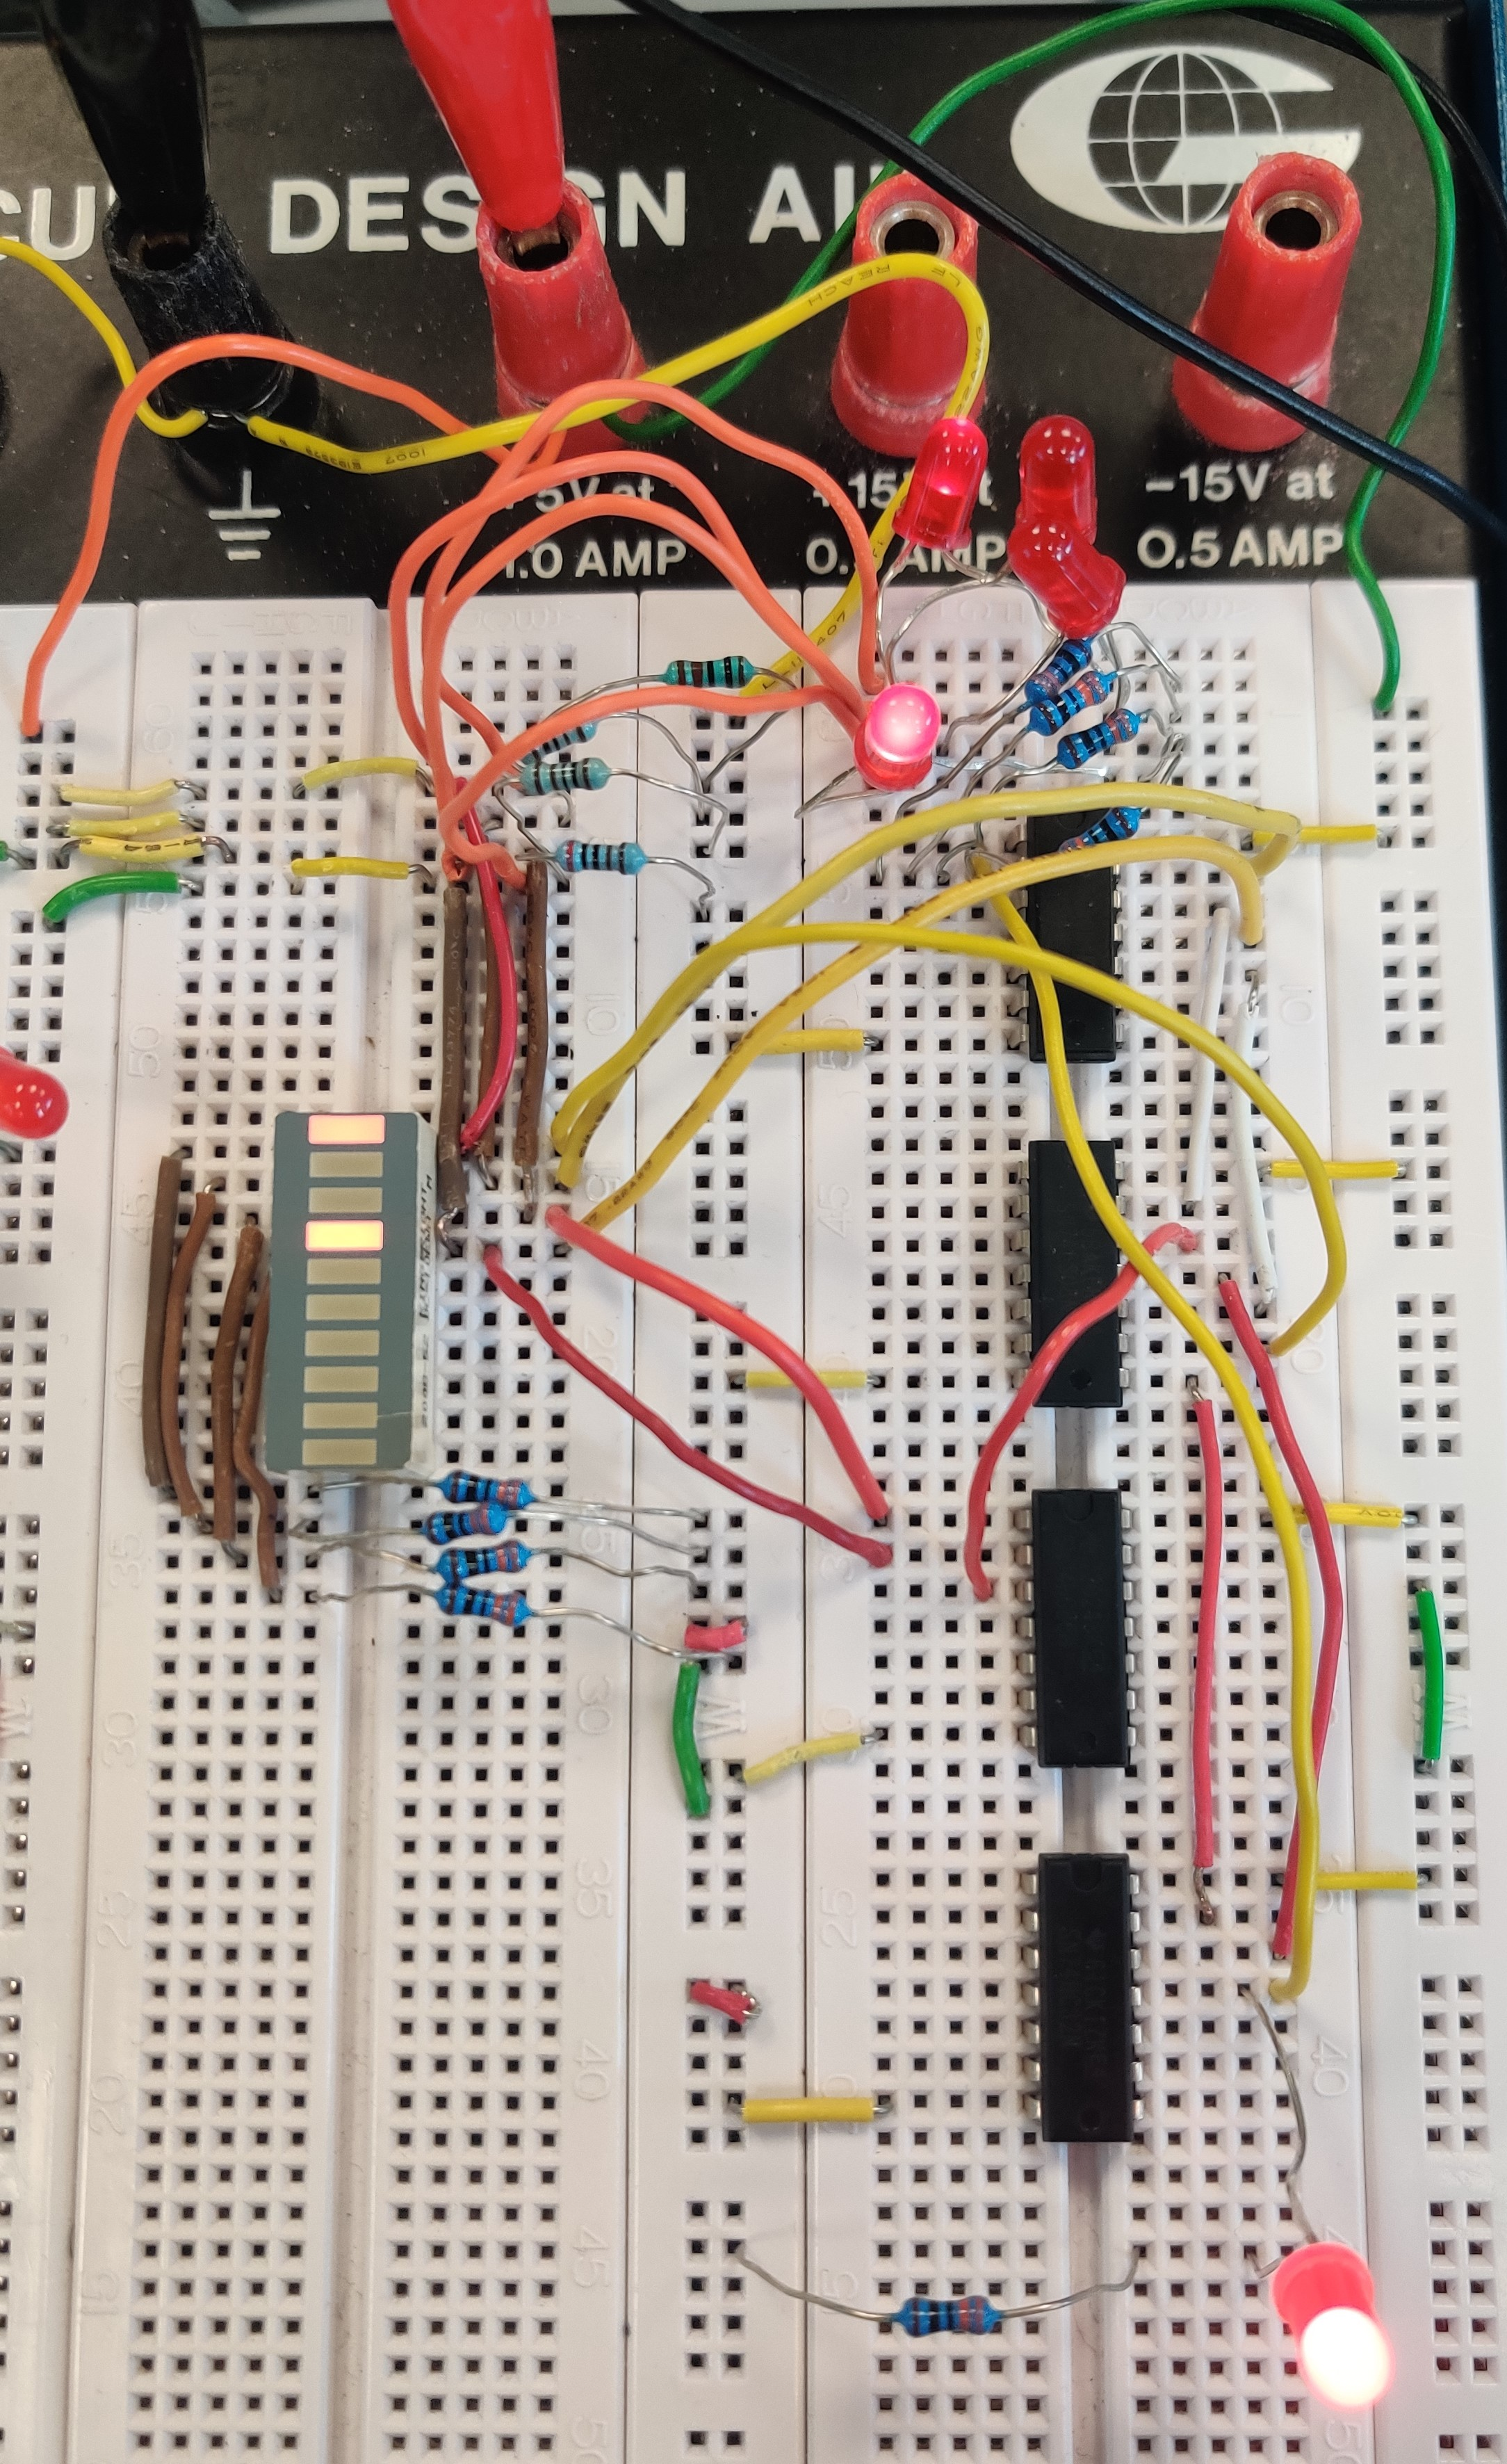
\includegraphics[width=8cm]{./images/logic_fitler_on.jpg}
  \caption{Input 1001 (Decimal 9) - Logic filter and motors $M_1$/$M_4$ are on }
  \label{fig:circuit_filter_on}
\end{figure}

In figure \ref{fig:circuit_filter_on} the inputs $S_1$ and $S_4$ are on. This corresponds to a the binary number 1001 or decimal 9. Looking
at table \ref{table:decimal} for input 9 motors $M_1$ and $M_4$ should be on. Exactly this can be seen: the LEDs corresponding to those
motors light up correctly. Additionally the filter indicator LED is also lighting up showing that the logic section correctly determined
the filter condition.

\begin{figure}[H]
  \centering
  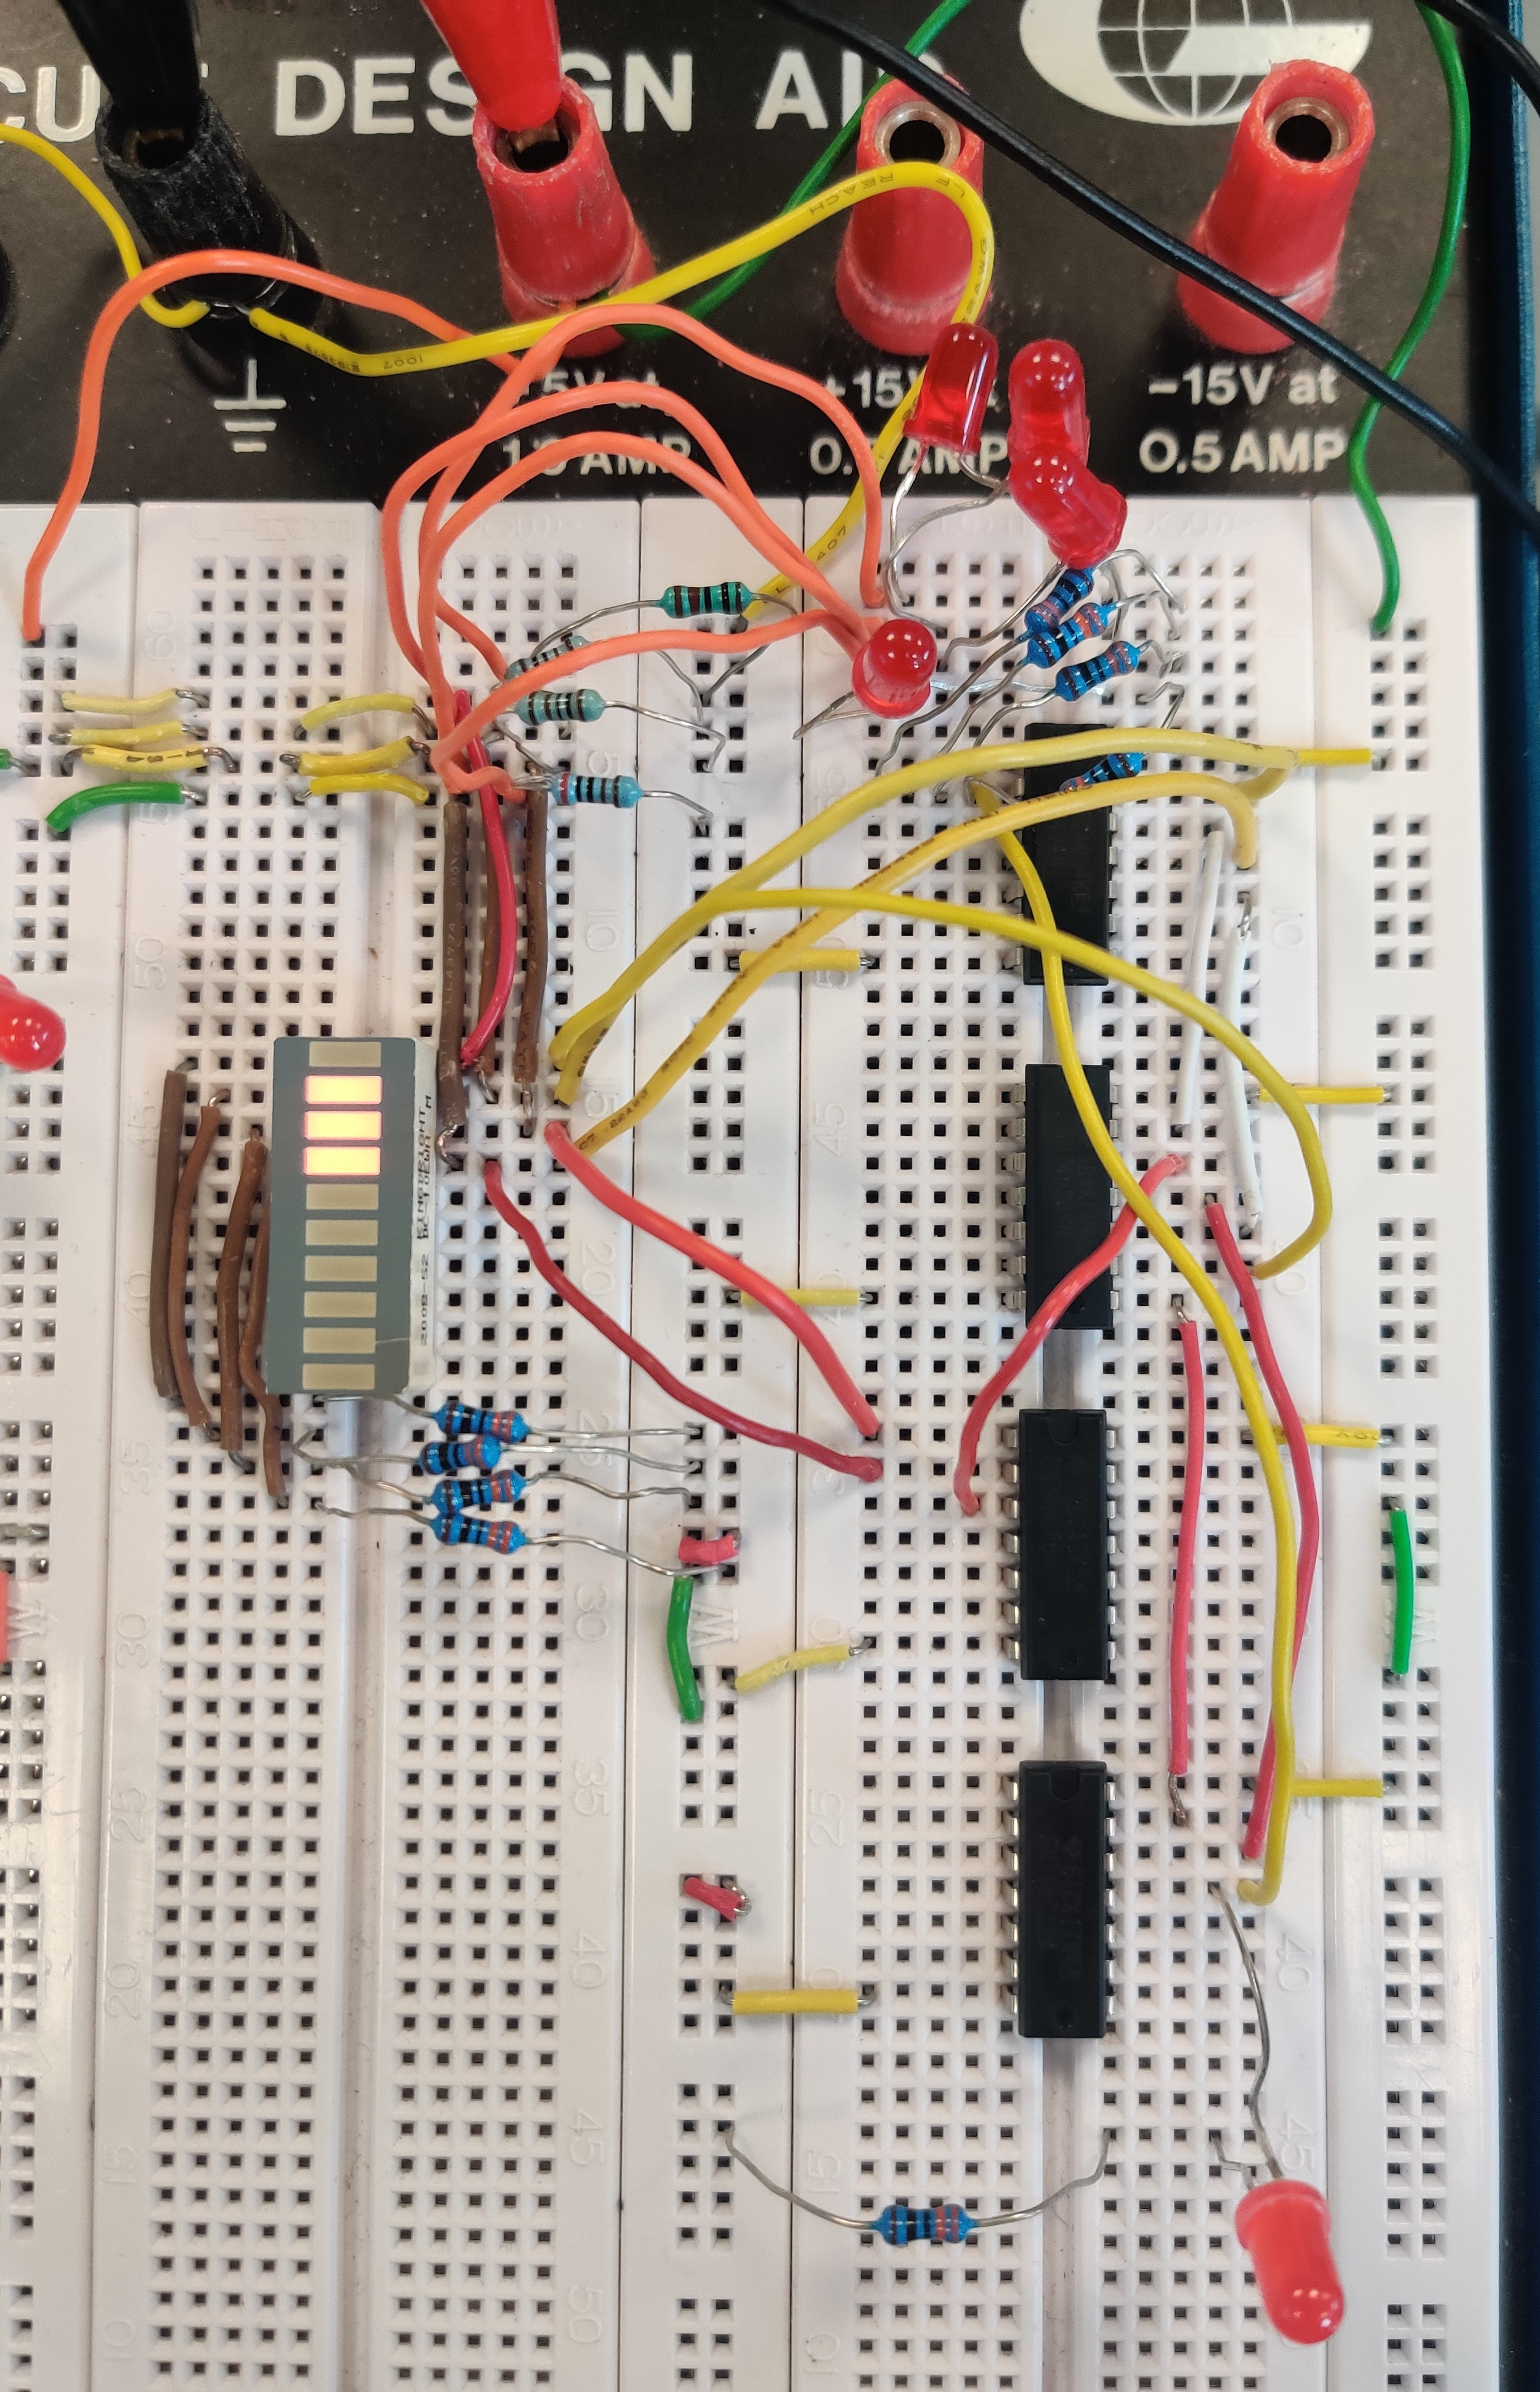
\includegraphics[width=8cm]{./images/logic_filter_off.jpg}
  \caption{Input 0111 (Decimal 7) - Logic filter and motors are off}
  \label{fig:circuit_filter_off}
\end{figure}

Figure \ref{fig:circuit_filter_off} shows one of the cases where the logic filter is LOW. Inputs $S_2$, $S_3$ and $S_4$ are on. This corresponds to a the binary number 0111 or decimal 7. Looking
at table \ref{table:decimal} for input 7 no motors should be on. This is what can be seen in the physical circuit, even though the inputs for
motors $M_{2-4}$ are HIGH the LEDs don't light up. This is because the logic filter correctly outputs LOW, thus disabling all LEDs as both
cathode and anode are HIGH (remember that the logic filter signal gets inverted).\\

The circuit shows the correct behavior for all 16 different input cases. Images showing all other cases are attached to the report.

\section{Conclusion}

The provided materials and components were suitable to implement and optimize a logical circuit given specific behavior requirements. To minimize
the number of components and therefore the complexity of the final design the boolean algebra simplifications outlined in the lab manual\autocite{ross} where
very effective. The usage of Multisim to model the circuit were both effective to flesh out a design and to verify that it was working before 
actually implementing it. Especially because of this the set time frame for the experiment was adequate. 

\printbibliography

\end{document}
